
%(BEGIN_QUESTION)

Hva menes med følgende begreper:

\begin{itemize}
\item Prosessvariabel
\item ProsessVerdi PV 
\item Manipulerende Variabel MV
\item Pådrag 
%\item Forstyrrelse 
\item Avviket e 
\end{itemize}


\begin{tikzpicture}
	\draw[step=0.5cm,gray!20,very thin]  grid (16,14) ;
\end{tikzpicture}

\vfil

\eject

\begin{tikzpicture}
	\draw[step=0.5cm,gray!20,very thin]  grid (16,23) ;
\end{tikzpicture}
%\underbar{file i00000}
%(END_QUESTION)





%(BEGIN_ANSWER)

\begin{itemize}
%\item Regulator - En enhet som har til oppgave å påvirke prosessen slik at den oppnår en ønsket tilstand (f.eks. et ønsket nivå eller en ønsket temperatur).
%\item Prosess - Det anlegget eller systemet som inngår i reguleringen.
\item Prosessvariabel - Den fysiske størrelsen i prosessen som skal reguleres (nivå, trykk, temperatur etc.)
\item ProsessVerdi PV - Den verdien prosessvariabelen til enhver tid har.
%\item Settpunkt SP - Den verdien vi ønsker at prosessvariabelen skal ha.
\item Manipulerende Variabel MV - Signalet som styrer pådragsorganet
%\item Forsyning - 
\item Pådrag - Det som er ment å variere prosessvariabelen. F.eks. væske inn i en nivåtank. 
%\item Belastning - Det som tas ut av prosessen ved konstant PV. Vil ha sammeverdi som pådraget. 
%\item Forstyrrelse - Forandringer som påvirker verdien til prosessvariabelen. 
\item Avviket e - Forskjellen mellom PV og SP (Direkte virkning PV-SP, Reverserende virkning SP-PV)
%\item Pådragsorgan - Den komponenten som styrer pådraget (f.eks. motoren
%i bilen som påvirker hastigheten, eller ventilen som påvirker nivået
%i tanken).
%\item Forstillingsenhet - I vårt eksempel med regulering av bilens hastighet,
%er forstillingsenheten forgasseren. Motoren er pådragsorganet i reguleringssløyfen.
%\item Auto og Manuell modus (Lukket- eller åpensløyfe). Om pådraget styres
%av regulatoren eller en manuell innstilt verdi. 
%\item LRV og URV ( Lover Range Value og Upper Range value, Laveste og høyeste
%verdi målesignalet kan ha.)
\end{itemize}

%(END_ANSWER)





%(BEGIN_NOTES)


%INDEX% Control, Definitions: (word or phrase here)

%(END_NOTES)



%(BEGIN_QUESTION)
% Copyright 2006, Tony R. Kuphaldt, released under the Creative Commons Attribution License (v 1.0)
% This means you may do almost anything with this work of mine, so long as you give me proper credit

Tegn grafen for utgangen  på denne regulatoren med bare p-ledd og direktevirkning. Den er stilt inn med følgende verdier:
\begin{itemize}[noitemsep]
	\item proporsjonalbånd 20\%
	\item bias 50 \%
\end{itemize}

%Graph the output of this proportional-only controller, assuming a proportional band value of 20\%, a bias value of 50\%, and a control action that is direct-acting:

$$\includegraphics[width=15.5cm]{i01469x01.eps}$$
Utregninger:\\

\begin{tikzpicture}
	\draw[step=0.5cm,gray!20,very thin]  grid (16,6) ;
\end{tikzpicture}
\vskip 20pt \vbox{\hrule \hbox{\strut \vrule{} {\bf Suggestions for Socratic discussion} \vrule} \hrule}

\begin{itemize}
\item{} Explain why this trend graph of the PV is unrealistic for a real process, but nevertheless useful for learning how a proportional-only controller is designed to respond to changes in PV.
\item{} How do you suppose the PV would {\it actually} respond in a real process to the conditions shown (or implied) in this trend?  Sketch what you would think would be a more realistic response assuming a properly-tuned proportional-only controller running in automatic mode.
\item{} Identify points on the trend where the PV exhibits a positive rate of change. 
\item{} Identify points on the trend where the PV exhibits a negative rate of change. 
\item{} Identify points on the trend where the PV exhibits zero change. 
\end{itemize}

\underbar{file i01469}
%(END_QUESTION)





%(BEGIN_ANSWER)

$$\includegraphics[width=15.5cm]{i01469x02.eps}$$

%(END_ANSWER)





%(BEGIN_NOTES)

With a proportional band value of 20\%, the gain will be equal to 5.

%INDEX% Control, proportional: graphing controller response

%(END_NOTES)



%(BEGIN_QUESTION)
% Copyright 2010, Tony R. Kuphaldt, released under the Creative Commons Attribution License (v 1.0)
% This means you may do almost anything with this work of mine, so long as you give me proper credit

Nivåreguleringen på denne steam kokeren har et problem. Vannivået i steambeholderen er under settpunktet. Regulatoren viser en PV på 42\% med et settpunkt på 50\%. Det har vert slik i flere timer, til tross for at operatøren har forsøkt å endre settpunkt. Kokeren går for fult og lager steam som normalt. 

%This boiler steam drum level control system has a problem.  The water level in the steam drum is below setpoint (as indicated by the controller display showing 42\% water level with a 50\% setpoint), and has been for the past several hours despite the operator's attempt to raise water level by raising the setpoint on the controller.  Meanwhile, the boiler is operating at full power, making steam at a normal rate of flow:

$$\includegraphics[width=15.5cm]{i01368x01.eps}$$

Identifiser sannsynligheten for hver av de spesifiserte feilene nedenfor. Du skal bare ta hensyn til en feil av gangen(ingen dobbeltfeil). Finn ut om hver av feilene kan være ansvarlig for symptomene i dette systemet. 

%Identify the likelihood of each specified fault for this system.  Consider each fault one at a time (i.e. no coincidental faults), determining whether or not each fault could independently account for {\it all} measurements and symptoms in this system.

% No blank lines allowed between lines of an \halign structure!
% I use comments (%) instead, so that TeX doesn't choke.

$$\vbox{\offinterlineskip
\halign{\strut
\vrule \quad\hfil # \ \hfil & 
\vrule \quad\hfil # \ \hfil & 
\vrule \quad\hfil # \ \hfil \vrule \cr
\noalign{\hrule}
%
% First row
{\bf Feil} & {\bf Mulig} & {\bf Umulig} \cr
%
\noalign{\hrule}
%
% Another row
LT kalibreringsfeil &  &  \cr
%
\noalign{\hrule}
%
% Another row
LY Kalibreringsfeil &  &  \cr
%
\noalign{\hrule}
%
% Another row
Defekt regulator &  &  \cr
%
\noalign{\hrule}
%
% Another row
Lavt trykk på luftforsyning &  &  \cr
%
\noalign{\hrule}
%
% Another row
Unormalt stor motstand i LT strømsløyfe &  &  \cr
%
\noalign{\hrule}
%
% Another row
Unormalt stor motstand i LY strømsløyfe &  &  \cr
%
\noalign{\hrule}
%
% Another row
Feedwater pumpe er slitt &  &  \cr
%
\noalign{\hrule}
%
% Another row
Regulatoren står i manuell modus. &  &  \cr
%
\noalign{\hrule}
} % End of \halign 
}$$ % End of \vbox

\underbar{file i01368}
%(END_QUESTION)





%(BEGIN_ANSWER)

Students are often surprised to find that a transmitter calibration error would {\it not} cause this problem.  A calibration error in the LT {\it would} cause the actual steam drum level to drift off setpoint, but with this being the only problem the controller would still register right on setpoint!

\vskip 10pt

A vital ``next test'' is to check the controller output, to see what it is trying to tell the valve to do.  It {\it should} be commanding the valve to open up.  If not, the controller definitely has some sort of problem (or is in manual mode).

%(END_ANSWER)





%(BEGIN_NOTES)

% No blank lines allowed between lines of an \halign structure!
% I use comments (%) instead, so that TeX doesn't choke.

$$\vbox{\offinterlineskip
\halign{\strut
\vrule \quad\hfil # \ \hfil & 
\vrule \quad\hfil # \ \hfil & 
\vrule \quad\hfil # \ \hfil \vrule \cr
\noalign{\hrule}
%
% First row
{\bf Fault} & {\bf Possible} & {\bf Impossible} \cr
%
\noalign{\hrule}
%
% Another row
LT calibration error &  & $\surd$ \cr
%
\noalign{\hrule}
%
% Another row
LY calibration error & ? &  \cr
%
\noalign{\hrule}
%
% Another row
Controller failed & $\surd$ &  \cr
%
\noalign{\hrule}
%
% Another row
Low air supply pressure & $\surd$ &  \cr
%
\noalign{\hrule}
%
% Another row
Excessive resistance in LT circuit &  & $\surd$ \cr
%
\noalign{\hrule}
%
% Another row
Excessive resistance in LY circuit &  & $\surd$ \cr
%
\noalign{\hrule}
%
% Another row
Feedwater pump worn & $\surd$ &  \cr
%
\noalign{\hrule}
%
% Another row
Controller in manual mode & ? &  \cr
%
\noalign{\hrule}
} % End of \halign 
}$$ % End of \vbox

An LY calibration error is possible only if the error is quite significant.  Otherwise, the controller will compensate for any modest valve errors through feedback.

The ``excessive resistance'' faults are not possible if we assume the extra resistance to be insufficient to cause the controller or transmitter to saturate.  Ideally, both current sources (LT and LIC) will fight as hard as they must to maintain proper current in each circuit, even with extra resistance.  However, if the extra resistance is very large, it would be possible for that resistance to force either current value to be less than it should be.

A controller in manual usually does not allow changes in setpoint due to the standard ``setpoint tracking'' feature.  If this feature is turned off, however, changes in setpoint are possible in manual mode.

\vskip 20pt \vbox{\hrule \hbox{\strut \vrule{} {\bf Virtual Troubleshooting} \vrule} \hrule}

This question is a good candidate for a ``Virtual Troubleshooting'' exercise.  Presenting the diagram to students, you first imagine in your own mind a particular fault in the system.  Then, you present one or more symptoms of that fault (something noticeable by an operator or other user of the system).  Students then propose various diagnostic tests to perform on this system to identify the nature and location of the fault, as though they were technicians trying to troubleshoot the problem.  Your job is to tell them what the result(s) would be for each of the proposed diagnostic tests, documenting those results where all the students can see.

During and after the exercise, it is good to ask students follow-up questions such as:

\begin{itemize}
\item{} What does the result of the last diagnostic test tell you about the fault?
\item{} Suppose the results of the last diagnostic test were different.  What then would that result tell you about the fault?
\item{} Is the last diagnostic test the best one we could do?
\item{} What would be the ideal order of tests, to diagnose the problem in as few steps as possible?
\end{itemize}

%(END_NOTES)



%(BEGIN_QUESTION)
% Copyright 2007, Tony R. Kuphaldt, released under the Creative Commons Attribution License (v 1.0)
% This means you may do almost anything with this work of mine, so long as you give me proper credit

Her vises sprangresponsen til en prosess med regulatoren i manuell modus. Regn ut prosessforsterkningen ($K$), tidskonstanten ($\tau$) og døtiden ($\theta$).


$$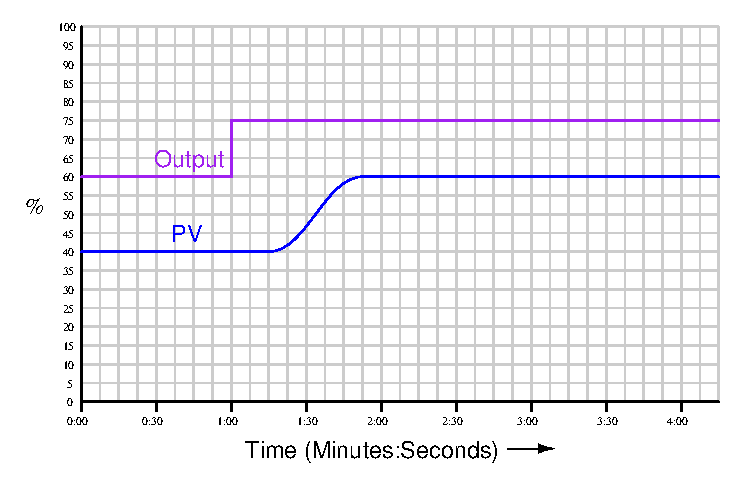
\includegraphics[width=15.5cm]{i01656x01.eps}$$

$K$ = \underbar{\hskip 50pt} \hskip 50pt $\tau$ = \underbar{\hskip 50pt} \hskip 50pt $\theta$ = \underbar{\hskip 50pt}

\vskip 10pt

Anta at vi gjør et mindre sprang i MV på prosessen, f.eks. 35\% istedenfor 15\%, hvilken effekt vil dette ha på $\tau$ og $\Theta$


\vskip 10pt


\underbar{file i01656}
%(END_QUESTION)





%(BEGIN_ANSWER)

$$\includegraphics[width=15.5cm]{i01656x02.eps}$$

\begin{itemize}
\item{}Steady-state gain ($K$) = 1.333
\vskip 5pt
\item{}Dead time ($L_R$) = 0.375 minutes
\vskip 5pt
\item{}Reaction rate ($R_R$) = 3.556\% / unit-minute
\end{itemize} 

\vskip 10pt

Note: the unit of ``unit-minute'' for reaction rate refers to reaction rate corrected for percentage of output step.  In other words, this is not the raw reaction rate figure, but rather the reaction rate per percent of output step.

\vskip 10pt

Ideally, there will be minimal effect on the apparent dead time ($L_R$) of the process, since such ``transport delays'' are usually unrelated to the manipulated variable.
 
The reaction rate ($R_R$) will also (ideally) remain constant.  Although the slope of the tangent line to the point of inflection on the PV curve will be steeper, this increase in steepness should be proportional to the increase in output step-change, resulting in an $R_R$ figure that is the same as with a lesser output step-change.

Of course, if the process gain changes throughout the PV range, then the reaction rate ($R_R$) will be affected by an increase in output step-change.

\vskip 10pt

$\tau$ = 0.375 minutes (approximately)

%(END_ANSWER)





%(BEGIN_NOTES)

{\it Calculating process gain:}

$K$ = $\Delta$PV / $\Delta$Output

$K$ = 20\% / 15\%

$K$ = 1.3333
 
\vskip 10pt

{\it Calculating apparent dead time:}

$L_R$ = (3 horizontal divisions on plot)(7.5 seconds / division)

$L_R$ = 22.5 seconds

$L_R$ = 0.375 minutes
 
\vskip 10pt
 
{\it Calculating reaction rate:}

$R_R$ = $\Delta$PV / (Lag time)($\Delta$Output)

$R_R$ = 20\% / (0.375 min)(15\%)

$R_R$ = 3.556\% / unit-minute
 
\vskip 10pt
 
NOTE: Some references suggest to calculate the reaction rate ($R_R$) as shown: the slope of the tangent line in \% per minute, per unit of output change.  Others omit the percent of output change, leading to an $R_R$ figure in units of \% per minute, but they assume an output change of only 1\% (1 unit), or else they incorporate the $\Delta$Output figure in a later equation when $R_R$ is used to calculate ideal PID constants.  

The tangent line slope is meaningless unless referenced to a specified change in output, since different step-changes in the output signal will lead to different rates of PV change per minute.

\vskip 10pt


Time constant ($\tau$) may be calculated two different ways:
 
\vskip 10pt

$\tau$ = Time required for PV to change 63.2\% from starting to final value (from the time the PV first starts to change -- no need to draw a reaction rate tangent line).
 
\vskip 10pt

$\tau$ = Time required for reaction rate tangent line to span full $\Delta$PV.

\vskip 10pt

NOTE: these two methods often produce significantly different results.  When in doubt, the best method to use is the first one, measuring the 63.2\% point on the vertical scale and then counting horizontal units of time.

%INDEX% Control, PID tuning: step change (output) revealing process gain
%INDEX% Control, PID tuning: step change (output) revealing process dead time
%INDEX% Control, PID tuning: step change (output) revealing process reaction rate

%(END_NOTES)



%(BEGIN_QUESTION)

Denne smelteovnen har et kaskadekoblet reguleringssystem der den primære regulatoren måler temperaturen i metallet som er smeltet og sekundær regulatoren regulerer temperaturen i ovnens vegger og tak. 

%This metal-melting furnace has a cascade control system, whereby a ``bath'' controller (sensing the temperature of the molten metal) acts as the primary, and a ``crown'' controller (sensing the temperature of the refractory wall and roof) acts as the secondary:

$$\includegraphics[width=15.5cm]{i01530x01.eps}$$

En dag blir sensorn i TT-1 defekt. Dette gjør at TT-1 sender et signal på 20.6mA. Hvilken effekt vil dette ha på reguleringssystemet?

%One day the crown thermocouple (the sensor for TT-1) goes bad, causing TT-1 to ``fail high'' with a 20.6 mA signal.  Determine the effect(s) this will have on the control system as a whole, and on the furnace temperature in particular.

\vskip 10pt


\begin{tikzpicture}
	\draw[step=0.5cm,gray!20,very thin]  grid (16,10) ;
\end{tikzpicture}

\vskip 20pt \vbox{\hrule \hbox{\strut \vrule{} {\bf Suggestions for Socratic discussion} \vrule} \hrule}

\begin{itemize}
\item{} Determine the necessary control actions (direct vs. reverse) for each controller in this system, assuming a signal-to-open valve.
\item{} Why do you think a cascade control strategy is used to control the burner?
\item{} For those who have studied thermocouples, what {\it type} (letter code) of thermocouple would you recommend for this application, assuming a crown temperature upwards of 1800 $^{o}$F?
\end{itemize}

\underbar{file i01530}
%(END_QUESTION)





%(BEGIN_ANSWER)

Not having the thermocouple fully inserted into the thermowell leads to additional {\it lag time}, as the air gap between the thermocouple tip and the thermowell bottom generates a time lag between the thermowell temperature and the thermocouple tip temperature. 

%(END_ANSWER)





%(BEGIN_NOTES)

A ``high burnout'' TT-1 would cause the furnace to cool down, as the temperature control system would ``think'' the furnace was too hot and take the necessary action of stopping heat input.

\vskip 10pt

Specifically, lag time in a feedback control system leads to greater phase shift, which may result in oscillation (cycling) given enough controller gain.  This is quite common in temperature control applications such as this, where the process itself may have only one dominant lag, allowing aggressive proportional action from the controller to achieve tight, fast control.  The addition of more lag times in a loop like that will often lead to oscillation, as the high gain of the controller now has enough phase shift to complement it and meet (or exceed) the Barkhausen criterion.

\vfil \eject

\noindent
{\bf Prep Quiz:}

An thermocouple improperly inserted into its thermowell can cause control problems by introducing what characteristic to the temperature control loop?

\begin{itemize}
\item{} Integral action
\vskip 10pt
\item{} Stiction
\vskip 10pt
\item{} Hysteresis
\vskip 10pt
\item{} Positive error
\vskip 10pt
\item{} Extra lag time
\vskip 10pt
\item{} Reverse action
\end{itemize}


%INDEX% Control, strategies: cascade with limits
%INDEX% Process: combustion furnace

%(END_NOTES)



%(BEGIN_QUESTION)
% Copyright 2007, Tony R. Kuphaldt, released under the Creative Commons Attribution License (v 1.0)
% This means you may do almost anything with this work of mine, so long as you give me proper credit

En gassfyrt varmeovn brukes til å varme opp en veskestrøm. En regulator brukes for å styre pådraget slik at temperauren på utgangen holdes konstant. 

%A gas-fired heater is used to increase the temperature of a liquid feed, working to hold that temperature constant at the value specified by a local setpoint (LSP):

$$\includegraphics[width=15.5cm]{i01776x01.eps}$$

\vskip 3cm 
Denne måten å sette opp et reguleringssystem er i de fleste tilfeller god nok, men det finnes bedre løsninger. Hva vil f.eks. skje om væskestrømmen som skal oppvarmes raskt stiger i temperatur? Regulatoren vil gjøre justeringer når denne forandringen har nådd utgangen av varmeovnen og temperaturtransmitteren (TT) har registrert det. 

En måte å forbedre dette systemet på er å innføre \textit{foroverkoblet} regulering. Modifiser systemet ved å bruke en temperaturtransmitter på væskestrømmen inn og koble denne som en foroverkoblng på systemet. 

%This simple control strategy may be adequate for most purposes, but there is room for improvement.  Consider, for instance, how the system will react if the temperature of the cold feed entering the heater suddenly increases.  Certainly, the temperature controller (TC) will take corrective action, but only after a rise in outlet temperature is sensed by the transmitter (TT).

%One way to improve the system's response to changes is to add {\it feedforward} control.  Modify the control scheme to include a feedforward signal from a feed temperature transmitter, and explain how the modified system will be better than the system in place now.

\vskip 20pt \vbox{\hrule \hbox{\strut \vrule{} {\bf Suggestions for Socratic discussion} \vrule} \hrule}

\begin{itemize}
\item{} Perhaps the single most common mistake students make when planning a feedforward system is mis-placing the location of the {\it summing} function block, where the load signal adds to the feedback control signal.  Explain why the load signal should always be added to the feedback controller {\it output} signal, and never to the feedback controller {\it PV} signal.
\item{} What do you suppose the heating ``coils'' look like in real life?
\item{} For those who have already studied temperature measurement, what kind(s) of temperature-sensing elements do you think could be used in this application?
\item{} Are there any loads unaccounted for in the requested feedforward control strategy?  If so, see if you can modify this control strategy to account for them as well.
\end{itemize}

\underbar{file i01776}
%(END_QUESTION)





%(BEGIN_ANSWER)

The following P\&IDs show {\it incorrect} implementations of feedforward to this process.  All of these incorrect solutions are commonly seen among students first learning about feedforward control.

\vskip 20pt


\noindent
{\bf Incorrect solution \#1:} A mysterious third input on the temperature controller (TC) is being used here.  Although some loop controllers do provide an input for a feedforward transmitter's signal, to sketch this as a solution does not demonstrate understanding of the feedforward strategy.  What needs to be shown is a more explicit function-block strategy whereby it is clear to see what the feedforward signal actually does to achieve its ends.

$$\includegraphics[width=15.5cm]{i01776x06.eps}$$

\vskip 10pt

\filbreak



\noindent
{\bf Incorrect solution \#2:} Here we see the feedforward signal being summed with the process variable signal before it enters the controller.  The reason this won't work has to do with the purpose of the temperature controller (TC) -- to maintain the outgoing product temperature at some operator-determined setpoint (local setpoint, or LSP).  If that controller isn't able to directly and accurately sense the product temperature (because that temperature signal is being added to a different temperature signal) then there is no way the controller will ever be able to hold the product temperature to setpoint.  In other words, summing the two temperature signals together effectively ``lies'' to the controller such that it never sees the real process variable, and therefore can never hold the real process variable stable at setpoint because it's operating on false information.

$$\includegraphics[width=15.5cm]{i01776x04.eps}$$



\vskip 10pt

\filbreak


\noindent
{\bf Incorrect solution \#3:} In this solution the feedforward signal is being used as a remote setpoint (RSP) to the temperature controller (TC), much like you would expect to see in a {\it ratio} control system.  The trouble with this solution is again related to the purpose of the temperature controller -- to maintain the outgoing product temperature at some operator-determined setpoint.  Here there is no operator-determined setpoint at all, but rather a setpoint determined solely by the incoming feed temperature.  

$$\includegraphics[width=15.5cm]{i01776x05.eps}$$

Furthermore, it makes absolutely no sense at all to have the controller's setpoint made equal to the incoming feed temperature.  If we tried this strategy, the controller would maintain a closed-valve condition at all times, because the surest way to maintain the outgoing product temperature at a setpoint value equal to the incoming feed temperature is to not heat it up at all!



\vskip 10pt

\filbreak


\noindent
{\bf Incorrect solution \#4:} Similar to the last incorrect solution (\#3), this one attempts to use the feedforward signal as {\it part} of a remote setpoint value (RSP) to the temperature controller (TC), while still maintaining an operator-determined local setpoint (LSP).  Here we still have the same fundamental problem as before -- so long as the feedforward signal modifies either the controller's view of the process variable (the outgoing product temperature) or its setpoint, the controller will be unable to perform its most basic function, to maintain the outgoing product temperature at some operator-determined setpoint.

$$\includegraphics[width=15.5cm]{i01776x07.eps}$$




\vskip 10pt

\filbreak


\noindent
{\bf Incorrect solution \#5:} This solution comes closer than all the others with regard to conceptual correctness, but there is no way for it to be practically implemented.  One cannot simple merge two different control signals together (i.e. the temperature controller's output signal somehow joining together with the feedforward signal).  Whether these signals are physical (e.g. two 4-20 mA DC currents or two digital fieldbus messages), or virtual (e.g. binary values inside of a control system such as a DCS), we need some sort of algorithm to combine them together.  The two signals will simply not merge together in any sensible way on their own.

$$\includegraphics[width=15.5cm]{i01776x08.eps}$$


%(END_ANSWER)





%(BEGIN_NOTES)

The mathematical signs adjacent to the two summer inputs are critically important, especially the negative sign ($-$) next to the feedforward signal input.  These signs dictate the direction of action for each of the signal pathways (feedback and feedforward):

$$\includegraphics[width=15.5cm]{i01776x03.eps}$$

Truth be told, the sign at the summer's feedback input may be set either positive or negative, so long as the controller (TC) is configured to a corresponding action (direct vs. reverse) such that the entire feedback loop has a negative characteristic.  For example, we could use a noninverting summer input combined with a reverse-acting controller, or alternatively an inverting summer input with a direct-acting controller.

The feedforward summer input, however, {\it absolutely must} be inverting because this is the only way we have of defining the feedforward path's direction of action.  Since a hotter feed temperature needs to result in a more-closed fuel valve, the feedforward action must be reverse, and the summer's sign at that input is the only means we have of establishing a reverse action for the feedforward path.



\vfil \eject

\noindent
{\bf Summary Quiz:}

Identify the consequence of the temperature transmitter failing ``high'' (e.g. 20 mA) in this control system:

$$\includegraphics[width=15.5cm]{i01776x02.eps}$$

\begin{itemize}
\item{} The natural gas supply pressure will increase
\vskip 5pt 
\item{} The feed flow rate into the heater will decrease
\vskip 5pt 
\item{} The feed (liquid) pressure will increase
\vskip 5pt 
\item{} The liquid exiting the heater will become too hot 
\vskip 5pt 
\item{} The feed flow rate into the heater will increase 
\vskip 5pt 
\item{} The liquid exiting the heater will become too cold
\end{itemize}

%INDEX% Control, strategies: feedforward
%INDEX% Process: heater (fired) (generic)

%(END_NOTES)


